
\begin{transitionframe}{Images/Transitions/TrifidNebula(Nasa)(PublicDomain).jpg}{black}
\textbf{Conclusions}
\end{transitionframe}



\begin{frame}{Summary of Results} \large

The (\alert{new}) insights we gained from experiments include:\\[.5em]
\begin{itemize}
\item Logic K sufficient for T1, C and T2 
\item Logic S5 \emph{not} needed for T3
\item \alert{Logic KB sufficient for T3 (not well known)}
\item \alert{We found a simpler new proof of C}
\item \alert{G\"odel's axioms (without conjunct $\phi(x)$ in D2) are inconsistent}
\item Scott's axioms are consistent
\item For T1, only half of A1 (A1a) is needed 
\item For T2, the other half (A1b) is needed
\end{itemize}
\end{frame}


\begin{frame}{Summary of Results} \large

\begin{itemize}
\item Contributions to the theorem proving community include \\[.5em]
\begin{itemize}
\item Powerful infrastructure for reasoning with QML
\item A (new?) natural deduction calculus for \\ higher-order (intuitionistic) modal logic
\item Difficult new benchmark problems for HOL provers
\item Huge media attention
\end{itemize}

\item Interesting bridge between CS, Philosophy and Theology

\item Major step towards \alert{Computer-assisted Theoretical Philosophy}
 \begin{itemize}
  \item see also Ed Zalta's \emph{Computational Metaphysics} project at Stanford University and John Rushby's formalization of Anselm's proof using PVS
  \item remember Leibniz' dictum --- \emph{Calculemus!}
  \end{itemize}
\end{itemize}
\end{frame}

\begin{frame}{Ongoing and Future Work} \large
\begin{itemize}
\item Formalize and verify other ontological arguments
  \begin{itemize}
  \item \ldots particularly the criticisms and improvements
  \end{itemize}
\item Experiment with other embeddings (e.g. varying domains)
\item Eliminate and introduce cuts
\end{itemize}
\end{frame}


\begin{frame}{Some Comments and Reactions}
\colorbox{gray}{
\includegraphics[width=.8\textwidth]{Images/Comments/Comment1}}\\[.7em]

\, \hfill \colorbox{gray}{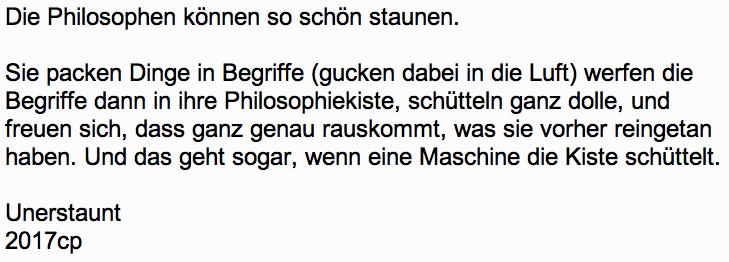
\includegraphics[width=.7\textwidth]{Images/Comments/Comment2}}\\[.7em]

\colorbox{gray}{
\includegraphics[width=.8\textwidth]{Images/Comments/Comment3}}\\[1em]

\, \hfill \ldots find more on the internet \ldots
\end{frame}

\begin{frame}[plain]
\colorbox{black}{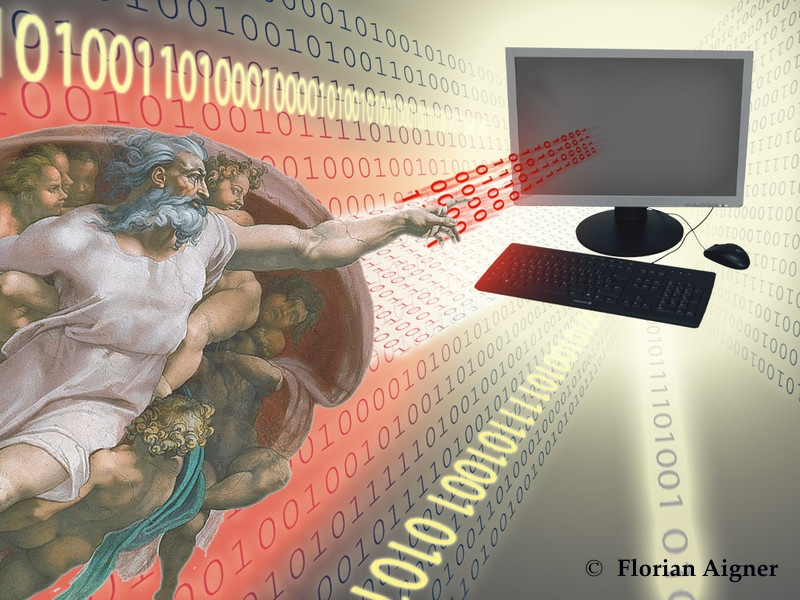
\includegraphics[width=\textwidth]{Images/Transitions/GodComputerC}}
\end{frame}

\begin{frame}{Licenses} \centering

\includegraphics[scale=0.5]{Images/CC-BY-SA.png}

\bigskip
\bigskip

\begin{center}
The following images used in these slides were obtained in commons.wikimedia.org and are licensed as follows:

\bigskip

CC-BY-SA:

ReligiousSymbols, PaganReligiousSymbols.

\bigskip

Public Domain: 

TrifidNebula
\end{center}
\end{frame}
